\documentclass[aspectratio=169, 11pt]{beamer}

% ==================== PACKAGES ====================
\usepackage{tikz}
\usetikzlibrary{shapes.geometric, arrows.meta, positioning, calc, fit, backgrounds, decorations.pathreplacing}
\usepackage{amsmath, amssymb}
\usepackage{booktabs}
\usepackage{graphicx}
\usepackage{xcolor}
\usepackage{fontawesome5}
\usepackage{listings}
\usepackage{multirow}
\usepackage{array}

% ==================== THEME ====================
\usetheme{Madrid}
\usecolortheme{seahorse}

% Custom colors
\definecolor{vflblue}{RGB}{41, 128, 185}
\definecolor{vflgreen}{RGB}{39, 174, 96}
\definecolor{vflred}{RGB}{231, 76, 60}
\definecolor{vflorange}{RGB}{243, 156, 18}
\definecolor{vflpurple}{RGB}{142, 68, 173}
\definecolor{vflgray}{RGB}{127, 140, 141}
\definecolor{lightbg}{RGB}{248, 249, 250}

\setbeamercolor{frametitle}{bg=vflblue, fg=white}
\setbeamercolor{title}{fg=vflblue}
\setbeamercolor{block title}{bg=vflblue, fg=white}
\setbeamercolor{block body}{bg=lightbg}
\setbeamercolor{block title alerted}{bg=vflred, fg=white}
\setbeamercolor{block title example}{bg=vflgreen, fg=white}

% ==================== TITLE INFO ====================
\title[E-VFU Framework]{\textbf{E-VFU: Multi-Attack Verification Framework}\\[0.3em] for Vertical Federated Unlearning}
\subtitle{A Comprehensive Approach to Verify Machine Unlearning in VFL}
\author{Gourab Biswas \and Fairuz}
\institute{Undergraduate Course in Machine Learning}
\date{\today}

% ==================== DOCUMENT ====================
\begin{document}

% ==================== TITLE SLIDE ====================
\begin{frame}
    \titlepage
\end{frame}

% ==================== OUTLINE ====================
\begin{frame}{Outline}
    \tableofcontents
\end{frame}

% ============================================================
% SECTION 1: INTRODUCTION
% ============================================================
\section{Introduction to Federated Learning}

\begin{frame}{What is Federated Learning?}
    \begin{center}
    \begin{tikzpicture}[scale=0.5, transform shape]
        % Central server
        \node[draw, circle, fill=vflblue!20, minimum size=2cm, line width=2pt] (server) at (0,0) {\faServer};
        \node[below=0.2cm of server, font=\bfseries] {Central Server};
        
        % Clients
        \foreach \i/\angle/\icon/\name in {1/90/\faHospital/Hospital, 2/210/\faUniversity/Bank, 3/330/\faBuilding/Company} {
            \node[draw, circle, fill=vflgreen!20, minimum size=1.5cm, line width=1.5pt] (c\i) at (\angle:3.5cm) {\icon};
            \node[font=\small] at (\angle:4.5cm) {\name};
        }
        
        % Arrows
        \foreach \i in {1,2,3} {
            \draw[-{Stealth}, thick, vflblue] (server) -- (c\i) node[midway, fill=white, font=\tiny] {Model};
            \draw[-{Stealth}, thick, vflgreen, dashed] (c\i) -- (server);
        }
    \end{tikzpicture}
    \end{center}
    
    \vspace{0.5em}
    \begin{alertblock}{\faLightbulb\ Key Insight}
        \centering
        \textit{``Don't move the data to the model; move the model to the data.''}
    \end{alertblock}
\end{frame}

\begin{frame}{Why Federated Learning?}
    \begin{columns}[T]
        \begin{column}{0.48\textwidth}
            \begin{block}{\faExclamationTriangle\ The Problem}
                \begin{itemize}
                    \item Organizations have valuable data
                    \item Privacy laws (GDPR, HIPAA) restrict sharing
                    \item Traditional ML requires centralized data
                \end{itemize}
            \end{block}
        \end{column}
        
        \begin{column}{0.48\textwidth}
            \begin{exampleblock}{\faCheck\ The Solution}
                \begin{itemize}
                    \item \faShieldAlt\ Privacy preserved
                    \item \faLock\ Data stays local
                    \item \faUsers\ Collaborative learning
                    \item \faBalanceScale\ Regulatory compliance
                \end{itemize}
            \end{exampleblock}
        \end{column}
    \end{columns}
\end{frame}

% ==================== HFL ====================
\begin{frame}{Horizontal Federated Learning (HFL)}
    \begin{columns}[T]
        \begin{column}{0.55\textwidth}
            \begin{block}{\faArrowsAltH\ Definition}
                \textbf{Same features, different samples}
            \end{block}
            
            \vspace{0.5em}
            \textbf{Example:} Multiple hospitals with patient records
            \begin{itemize}
                \item Same medical tests (features)
                \item Different patients (samples)
            \end{itemize}
            
            \vspace{0.5em}
            \begin{alertblock}{Data Distribution}
                Each client holds a \textbf{horizontal slice} of the full dataset
            \end{alertblock}
        \end{column}
        
        \begin{column}{0.42\textwidth}
            \begin{center}
            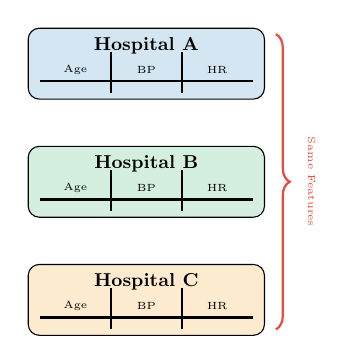
\begin{tikzpicture}[scale=0.75, transform shape]
                \foreach \y/\name/\color in {2/Hospital A/vflblue, 0/Hospital B/vflgreen, -2/Hospital C/vflorange} {
                    \draw[fill=\color!20, rounded corners] (-2,\y-0.6) rectangle (2,\y+0.6);
                    \node[font=\small\bfseries] at (0,\y+0.3) {\name};
                    \foreach \r in {-0.3} {
                        \draw[thick] (-1.8,\y+\r) -- (1.8,\y+\r);
                    }
                    \foreach \c in {-0.6, 0.6} {
                        \draw[thick] (\c,\y-0.5) -- (\c,\y+0.2);
                    }
                    \node[font=\tiny] at (-1.2, \y-0.1) {Age};
                    \node[font=\tiny] at (0, \y-0.1) {BP};
                    \node[font=\tiny] at (1.2, \y-0.1) {HR};
                }
                
                \draw[decorate, decoration={brace, amplitude=5pt, raise=2pt}, thick, vflred] (2.1,2.5) -- (2.1,-2.5);
                \node[font=\tiny, rotate=-90, vflred] at (2.8,0) {Same Features};
            \end{tikzpicture}
            \end{center}
        \end{column}
    \end{columns}
\end{frame}

% ==================== VFL ====================
\begin{frame}{Vertical Federated Learning (VFL)}
    \begin{columns}[T]
        \begin{column}{0.55\textwidth}
            \begin{block}{\faArrowsAltV\ Definition}
                \textbf{Same samples, different features}
            \end{block}
            
            \vspace{0.5em}
            \textbf{Example:} Bank + Hospital + Government
            \begin{itemize}
                \item Same individuals (samples)
                \item Different information (features)
            \end{itemize}
            
            \vspace{0.5em}
            \begin{exampleblock}{Data Distribution}
                Each party holds a \textbf{vertical slice} (different columns)
            \end{exampleblock}
        \end{column}
        
        \begin{column}{0.42\textwidth}
            \begin{center}
            \begin{tikzpicture}[scale=0.75, transform shape]
                \draw[fill=lightbg, rounded corners] (-2.5,-1.5) rectangle (2.5,1.5);
                
                \draw[fill=vflblue!30] (-2.4,-1.4) rectangle (-0.5,1.4);
                \node[font=\tiny\bfseries, vflblue] at (-1.45,1.1) {Bank};
                \node[font=\tiny] at (-1.45,0.5) {Income};
                \node[font=\tiny] at (-1.45,0) {Credit};
                \node[font=\tiny] at (-1.45,-0.5) {Debt};
                
                \draw[fill=vflgreen!30] (-0.4,-1.4) rectangle (1.3,1.4);
                \node[font=\tiny\bfseries, vflgreen] at (0.45,1.1) {Hospital};
                \node[font=\tiny] at (0.45,0.5) {Age};
                \node[font=\tiny] at (0.45,0) {BMI};
                \node[font=\tiny] at (0.45,-0.5) {BP};
                
                \draw[fill=vflorange!30] (1.4,-1.4) rectangle (2.4,1.4);
                \node[font=\tiny\bfseries, vflorange] at (1.9,1.1) {Gov.};
                \node[font=\tiny] at (1.9,0) {\faTag};
                \node[font=\tiny] at (1.9,-0.5) {Label};
                
                \draw[decorate, decoration={brace, amplitude=5pt, raise=2pt}, thick, vflpurple] (-2.5,-1.7) -- (2.5,-1.7);
                \node[font=\tiny, vflpurple] at (0,-2.3) {Same Samples (linked by ID)};
            \end{tikzpicture}
            \end{center}
        \end{column}
    \end{columns}
    
    \vspace{0.5em}
    \centering
    \colorbox{yellow!20}{\textbf{Our Focus: Vertical Federated Learning (VFL)}}
\end{frame}

% ============================================================
% SECTION 2: WHY UNLEARNING?
% ============================================================
\section{The Need for Machine Unlearning}

\begin{frame}{The Unlearning Problem}
    \begin{center}
    \begin{tikzpicture}[scale=0.85, transform shape]
        % Brain/Model
        \node[draw, circle, fill=vflblue!20, minimum size=2.5cm, line width=2pt] (model) at (0,0) {\faBrain};
        \node[below=0.3cm of model, font=\bfseries] {Trained Model};
        
        % Data points around
        \foreach \i/\angle/\col in {1/45/vflgreen, 2/90/vflgreen, 3/135/vflgreen, 4/180/vflred, 5/225/vflgreen, 6/270/vflgreen, 7/315/vflgreen} {
            \node[draw, circle, fill=\col!40, minimum size=0.6cm, font=\tiny] (d\i) at (\angle:2.2cm) {\faUser};
        }
        
        % Highlight the one to remove
        \draw[very thick, vflred, dashed] (d4) circle (0.5cm);
        \node[font=\small, vflred, left=0.5cm of d4] {Remove me!};
        
        % Arrow showing unlearning
        \draw[-{Stealth}, ultra thick, vflred] (d4) -- (model);
    \end{tikzpicture}
    \end{center}
    
    \vspace{0.5em}
    \begin{alertblock}{\faExclamationTriangle\ The Challenge}
        \centering
        Once a model learns from data, it \textbf{remembers} that data!\\
        How do we make the model ``forget'' specific data points?
    \end{alertblock}
\end{frame}

\begin{frame}{Why Do We Need Unlearning?}
    \begin{columns}[T]
        \begin{column}{0.48\textwidth}
            \begin{block}{\faGavel\ Legal Requirements}
                \begin{itemize}
                    \item \textbf{GDPR Article 17}:\\``Right to be Forgotten''
                    \item Users can request data deletion
                    \item Model must behave \textit{as if} it never saw the data
                \end{itemize}
            \end{block}
        \end{column}
        
        \begin{column}{0.48\textwidth}
            \begin{block}{\faBug\ Other Scenarios}
                \begin{itemize}
                    \item Remove poisoned/malicious data
                    \item Correct training errors
                    \item Data retention policies
                    \item Client leaves federation
                \end{itemize}
            \end{block}
        \end{column}
    \end{columns}
\end{frame}

\begin{frame}{Naive vs. Smart Unlearning}
    \begin{columns}[T]
        \begin{column}{0.48\textwidth}
            \begin{alertblock}{\faTimes\ Naive: Retrain from Scratch}
            \end{alertblock}
            
            \begin{center}
            \begin{tikzpicture}[scale=0.7, transform shape]
                \node[draw, rectangle, fill=vflblue!20, minimum width=2cm, minimum height=0.8cm] (data) at (0,2) {Full Data};
                \draw[-{Stealth}, thick] (0,1.5) -- (0,0.8);
                \node[draw, rectangle, fill=vflgreen!20, minimum width=1.5cm, minimum height=0.8cm] (remain) at (0,0.3) {Remaining};
                \draw[-{Stealth}, thick] (0,-0.2) -- (0,-1);
                \node[draw, circle, fill=vflorange!30, minimum size=1cm] (model) at (0,-1.5) {\faBrain};
                \node[font=\scriptsize, vflred] at (2.2,-0.6) {\faClock\ Hours/Days!};
            \end{tikzpicture}
            \end{center}
            
            \begin{itemize}
                \item[\faTimes] Extremely slow
                \item[\faTimes] Computationally expensive
            \end{itemize}
        \end{column}
        
        \begin{column}{0.48\textwidth}
            \begin{exampleblock}{\faCheck\ Smart: Machine Unlearning}
            \end{exampleblock}
            
            \begin{center}
            \begin{tikzpicture}[scale=0.7, transform shape]
                \node[draw, circle, fill=vflblue!30, minimum size=1cm] (model1) at (0,2) {\faBrain};
                \node[font=\tiny, right] at (0.6,2) {Original};
                \draw[-{Stealth}, thick, vflred] (model1) -- (0,0.8);
                \node[draw, circle, fill=vflgreen!30, minimum size=1cm] (model2) at (0,0.3) {\faBrain};
                \node[font=\tiny, right] at (0.6,0.3) {Unlearned};
                \node[font=\scriptsize, vflgreen] at (2.2,1.4) {\faClock\ Minutes!};
            \end{tikzpicture}
            \end{center}
            
            \begin{itemize}
                \item[\faCheck] Fast and efficient
                \item[\faCheck] Minimal utility loss
            \end{itemize}
        \end{column}
    \end{columns}
\end{frame}

% ============================================================
% SECTION 3: VFL ARCHITECTURE
% ============================================================
\section{Our VFL Architecture}

\begin{frame}{VFL Split Learning Architecture}
    \begin{center}
    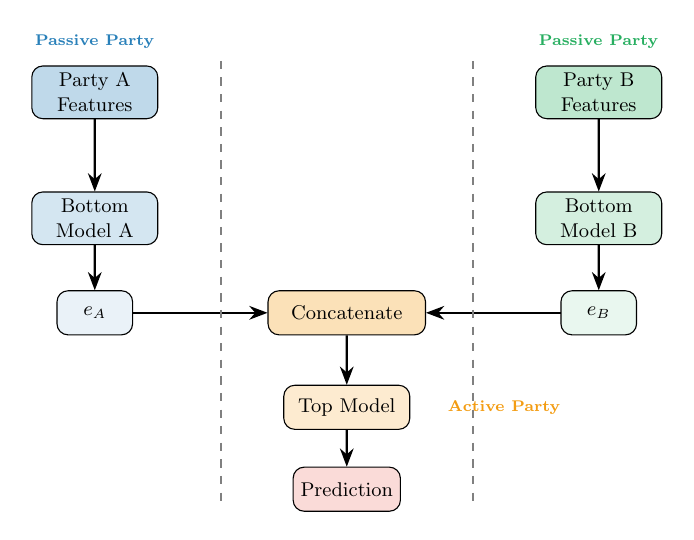
\begin{tikzpicture}[scale=0.8, transform shape,
        box/.style={draw, rounded corners, minimum width=2cm, minimum height=0.7cm, align=center, font=\small},
        arrow/.style={-{Stealth}, thick}]
        
        % Party A (Left)
        \node[box, fill=vflblue!30] (dataA) at (-4, 2) {Party A\\Features};
        \node[box, fill=vflblue!20] (bottomA) at (-4, 0) {Bottom\\Model A};
        \node[box, fill=vflblue!10, minimum width=1.2cm] (embA) at (-4, -1.5) {$e_A$};
        
        % Party B (Right)
        \node[box, fill=vflgreen!30] (dataB) at (4, 2) {Party B\\Features};
        \node[box, fill=vflgreen!20] (bottomB) at (4, 0) {Bottom\\Model B};
        \node[box, fill=vflgreen!10, minimum width=1.2cm] (embB) at (4, -1.5) {$e_B$};
        
        % Top Model (Center)
        \node[box, fill=vflorange!30, minimum width=2.5cm] (concat) at (0, -1.5) {Concatenate};
        \node[box, fill=vflorange!20, minimum width=2cm] (top) at (0, -3) {Top Model};
        \node[box, fill=vflred!20, minimum width=1.5cm] (output) at (0, -4.3) {Prediction};
        
        % Arrows
        \draw[arrow] (dataA) -- (bottomA);
        \draw[arrow] (dataB) -- (bottomB);
        \draw[arrow] (bottomA) -- (embA);
        \draw[arrow] (bottomB) -- (embB);
        \draw[arrow] (embA) -- (concat);
        \draw[arrow] (embB) -- (concat);
        \draw[arrow] (concat) -- (top);
        \draw[arrow] (top) -- (output);
        
        % Annotations
        \node[font=\scriptsize, vflblue] at (-4, 2.8) {\textbf{Passive Party}};
        \node[font=\scriptsize, vflgreen] at (4, 2.8) {\textbf{Passive Party}};
        \node[font=\scriptsize, vflorange] at (2.5, -3) {\textbf{Active Party}};
        
        % Privacy boundary
        \draw[dashed, thick, gray] (-2, 2.5) -- (-2, -4.5);
        \draw[dashed, thick, gray] (2, 2.5) -- (2, -4.5);
    \end{tikzpicture}
    \end{center}
\end{frame}

\begin{frame}{Architecture Components}
    \begin{columns}[T]
        \begin{column}{0.32\textwidth}
            \begin{block}{\faCubes\ Bottom Models}
                \begin{itemize}
                    \item One per party
                    \item Processes local features
                    \item Outputs embedding
                \end{itemize}
                
                \vspace{0.3em}
                \small
                Linear(64) $\rightarrow$ ReLU $\rightarrow$\\
                BatchNorm $\rightarrow$ Dropout $\rightarrow$\\
                Linear(32)
            \end{block}
        \end{column}
        
        \begin{column}{0.32\textwidth}
            \begin{block}{\faExchangeAlt\ Embeddings}
                \begin{itemize}
                    \item 32-dimensional vectors
                    \item Shared between parties
                    \item Raw data stays local!
                \end{itemize}
                
                \vspace{0.3em}
                \small
                Privacy-preserving\\
                communication layer
            \end{block}
        \end{column}
        
        \begin{column}{0.32\textwidth}
            \begin{block}{\faSitemap\ Top Model}
                \begin{itemize}
                    \item Active party only
                    \item Combines embeddings
                    \item Makes prediction
                \end{itemize}
                
                \vspace{0.3em}
                \small
                Concat $\rightarrow$ Linear(64) $\rightarrow$\\
                ReLU $\rightarrow$ Linear(1) $\rightarrow$\\
                Sigmoid
            \end{block}
        \end{column}
    \end{columns}
    
    \vspace{0.5em}
    \begin{center}
        \colorbox{yellow!20}{\small \textbf{Training:} BCE Loss + Adam (lr=0.001)}
    \end{center}
\end{frame}

% ============================================================
% SECTION 4: UNLEARNING METHODS
% ============================================================
\section{VFL Unlearning Methods}

\begin{frame}{Three Unlearning Approaches}
    \begin{center}
    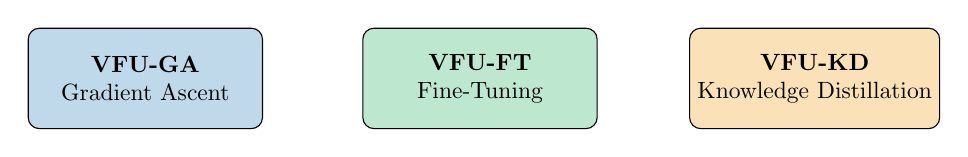
\begin{tikzpicture}[scale=0.85, transform shape]
        % VFU-GA
        \node[draw, rounded corners, fill=vflblue!30, minimum width=3.5cm, minimum height=1.5cm, align=center] (ga) at (-5, 0) {\textbf{VFU-GA}\\Gradient Ascent};
        
        % VFU-FT
        \node[draw, rounded corners, fill=vflgreen!30, minimum width=3.5cm, minimum height=1.5cm, align=center] (ft) at (0, 0) {\textbf{VFU-FT}\\Fine-Tuning};
        
        % VFU-KD
        \node[draw, rounded corners, fill=vflorange!30, minimum width=3.5cm, minimum height=1.5cm, align=center] (kd) at (5, 0) {\textbf{VFU-KD}\\Knowledge Distillation};
    \end{tikzpicture}
    \end{center}
    
    \vspace{1em}
    \begin{table}[]
        \centering
        \begin{tabular}{lccc}
            \toprule
            \textbf{Aspect} & \textbf{VFU-GA} & \textbf{VFU-FT} & \textbf{VFU-KD} \\
            \midrule
            Speed & \textcolor{vflgreen}{\faCheckCircle\ Fast} & \textcolor{vflorange}{\faCircle\ Medium} & \textcolor{vflred}{\faTimesCircle\ Slow} \\
            Utility & \textcolor{vflorange}{\faCircle\ Medium} & \textcolor{vflgreen}{\faCheckCircle\ Good} & \textcolor{vflgreen}{\faCheckCircle\ Best} \\
            Forgetting & \textcolor{vflgreen}{\faCheckCircle\ Strong} & \textcolor{vflorange}{\faCircle\ Medium} & \textcolor{vflgreen}{\faCheckCircle\ Strong} \\
            \bottomrule
        \end{tabular}
    \end{table}
\end{frame}

\begin{frame}{VFU-GA: Gradient Ascent}
    \begin{columns}[T]
        \begin{column}{0.55\textwidth}
            \begin{block}{\faLightbulb\ Core Idea}
                Training uses \textbf{gradient descent} to minimize loss.\\
                Unlearning uses \textbf{gradient ascent} to maximize loss!
            \end{block}
            
            \vspace{0.5em}
            \textbf{Standard Training:}
            \[
            \theta_{t+1} = \theta_t - \eta \cdot \nabla_\theta \mathcal{L}
            \]
            
            \textbf{Gradient Ascent Unlearning:}
            \[
            \theta_{t+1} = \theta_t \textcolor{vflred}{\mathbf{+}} \eta \cdot \nabla_\theta \mathcal{L}
            \]
        \end{column}
        
        \begin{column}{0.42\textwidth}
            \begin{center}
            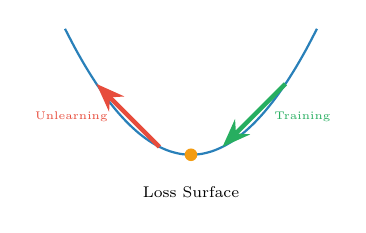
\begin{tikzpicture}[scale=0.8, transform shape]
                \draw[thick, domain=-2:2, smooth, variable=\x, vflblue] plot ({\x}, {0.5*\x*\x});
                \node[font=\scriptsize] at (0, -0.6) {Loss Surface};
                
                \draw[-{Stealth}, ultra thick, vflgreen] (1.5, 1.125) -- (0.5, 0.125);
                \node[font=\tiny, vflgreen, right] at (1.2, 0.6) {Training};
                
                \draw[-{Stealth}, ultra thick, vflred] (-0.5, 0.125) -- (-1.5, 1.125);
                \node[font=\tiny, vflred, left] at (-1.2, 0.6) {Unlearning};
                
                \fill[vflorange] (0, 0) circle (0.1);
            \end{tikzpicture}
            \end{center}
        \end{column}
    \end{columns}
\end{frame}

\begin{frame}{VFU-GA: Implementation Details}
    \begin{block}{\faCode\ Our Implementation}
        \begin{itemize}
            \item Negate the loss: \texttt{loss = -criterion(output, target)}
            \item Run for \textbf{10 epochs} on target samples only
            \item Learning rate: 0.001 (same as training)
        \end{itemize}
    \end{block}
    
    \vspace{0.5em}
    \begin{columns}[T]
        \begin{column}{0.48\textwidth}
            \begin{exampleblock}{\faCheck\ Pros}
                \begin{itemize}
                    \item Fastest method
                    \item Simple to implement
                    \item No additional data needed
                \end{itemize}
            \end{exampleblock}
        \end{column}
        \begin{column}{0.48\textwidth}
            \begin{alertblock}{\faTimes\ Cons}
                \begin{itemize}
                    \item Can hurt model utility
                    \item Too many epochs = catastrophic
                    \item Leaves detectable traces (FUMA)
                \end{itemize}
            \end{alertblock}
        \end{column}
    \end{columns}
\end{frame}

\begin{frame}{VFU-FT: Fine-Tuning}
    \begin{center}
    \begin{tikzpicture}[scale=0.8, transform shape]
        % Original model
        \node[draw, circle, fill=vflblue!30, minimum size=1.8cm] (model1) at (-4, 0) {\faBrain};
        \node[below=0.2cm of model1, font=\bfseries] {Original Model};
        
        % Data
        \node[draw, rectangle, fill=vflred!30, dashed, minimum width=1.5cm] (forget) at (0, 1.5) {Forget Data};
        \node[draw, rectangle, fill=vflgreen!30, minimum width=2cm] (retain) at (0, -1.5) {Retain Data};
        
        % Cross out forget
        \draw[very thick, vflred] (-0.6, 1.8) -- (0.6, 1.2);
        \draw[very thick, vflred] (-0.6, 1.2) -- (0.6, 1.8);
        
        % Arrow
        \draw[-{Stealth}, ultra thick, vflgreen] (model1) -- (4, 0) node[midway, above, font=\small] {Continue training};
        \draw[-{Stealth}, thick, vflgreen] (retain) -- (2, -0.5);
        
        % New model
        \node[draw, circle, fill=vflgreen!30, minimum size=1.8cm] (model2) at (4, 0) {\faBrain};
        \node[below=0.2cm of model2, font=\bfseries] {Unlearned Model};
    \end{tikzpicture}
    \end{center}
    
    \vspace{0.5em}
    \begin{block}{\faLightbulb\ Core Idea}
        Simply continue training on \textbf{remaining data only} (excluding target samples).\\
        The model gradually ``overwrites'' its memory of the forgotten data.
    \end{block}
\end{frame}

\begin{frame}{VFU-FT: Implementation Details}
    \begin{block}{\faCode\ Our Implementation}
        \begin{itemize}
            \item Remove target indices from training set
            \item Continue training for \textbf{20 epochs}
            \item Learning rate: 0.0005 (lower than initial training)
            \item Batch size: 256
        \end{itemize}
    \end{block}
    
    \vspace{0.5em}
    \begin{columns}[T]
        \begin{column}{0.48\textwidth}
            \begin{exampleblock}{\faCheck\ Pros}
                \begin{itemize}
                    \item Good utility preservation
                    \item Stable training
                    \item Natural forgetting process
                \end{itemize}
            \end{exampleblock}
        \end{column}
        \begin{column}{0.48\textwidth}
            \begin{alertblock}{\faTimes\ Cons}
                \begin{itemize}
                    \item Slower than VFU-GA
                    \item Weaker forgetting guarantee
                    \item May retain some information
                \end{itemize}
            \end{alertblock}
        \end{column}
    \end{columns}
\end{frame}

\begin{frame}{VFU-KD: Knowledge Distillation}
    \begin{center}
    \begin{tikzpicture}[scale=0.8, transform shape,
        model/.style={draw, circle, minimum size=1.8cm, font=\small}]
        
        % Teacher model
        \node[model, fill=vflblue!30] (teacher) at (-3, 1) {\faBrain};
        \node[below=0.2cm of teacher, font=\bfseries, vflblue] {Teacher};
        \node[below=0.7cm of teacher, font=\tiny] {(Original Model)};
        
        % Student model
        \node[model, fill=vflgreen!30] (student) at (3, 1) {\faBrain};
        \node[below=0.2cm of student, font=\bfseries, vflgreen] {Student};
        \node[below=0.7cm of student, font=\tiny] {(New Model)};
        
        % Data
        \node[draw, rectangle, rounded corners, fill=vflorange!30, minimum width=2.5cm] (retain) at (0, -1.5) {Retain Data Only};
        \node[draw, rectangle, rounded corners, fill=vflred!30, dashed, minimum width=2cm] (forget) at (-5, -1.5) {Forget Data};
        
        % Cross out
        \draw[very thick, vflred] (-5.8, -1.2) -- (-4.2, -1.8);
        \draw[very thick, vflred] (-5.8, -1.8) -- (-4.2, -1.2);
        
        % Arrows
        \draw[-{Stealth}, thick, vflblue] (retain) -- (teacher);
        \draw[-{Stealth}, thick, vflgreen] (retain) -- (student);
        \draw[-{Stealth}, ultra thick, vflpurple, dashed] (teacher) -- (student) node[midway, above, font=\small] {Knowledge};
    \end{tikzpicture}
    \end{center}
\end{frame}

\begin{frame}{VFU-KD: Loss Function}
    \begin{center}
    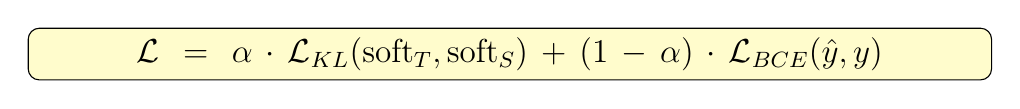
\begin{tikzpicture}
        \node[draw, rounded corners, fill=yellow!20, text width=12cm, align=center, font=\large] {
            $\mathcal{L} = \alpha \cdot \mathcal{L}_{KL}(\text{soft}_T, \text{soft}_S) + (1-\alpha) \cdot \mathcal{L}_{BCE}(\hat{y}, y)$
        };
    \end{tikzpicture}
    \end{center}
    
    \vspace{0.5em}
    \begin{block}{\faInfoCircle\ Components}
        \begin{itemize}
            \item $\mathcal{L}_{KL}$: KL divergence between teacher and student soft predictions
            \item $\mathcal{L}_{BCE}$: Binary cross-entropy with ground truth labels
            \item $\alpha = 0.5$: Balance between teacher knowledge and true labels
            \item Temperature $T = 2.0$: Softens probability distributions
        \end{itemize}
    \end{block}
\end{frame}

\begin{frame}{VFU-KD: Implementation Details}
    \begin{block}{\faCode\ Our Implementation}
        \begin{itemize}
            \item Create \textbf{new student model} (same architecture)
            \item Teacher generates soft labels on retain data only
            \item Train student for \textbf{30 epochs}
            \item Combined loss: 50\% KL + 50\% BCE
        \end{itemize}
    \end{block}
    
    \vspace{0.5em}
    \begin{columns}[T]
        \begin{column}{0.48\textwidth}
            \begin{exampleblock}{\faCheck\ Pros}
                \begin{itemize}
                    \item Best utility preservation
                    \item Strong forgetting guarantee
                    \item Student never sees target data
                \end{itemize}
            \end{exampleblock}
        \end{column}
        \begin{column}{0.48\textwidth}
            \begin{alertblock}{\faTimes\ Cons}
                \begin{itemize}
                    \item Slowest method
                    \item Requires full retraining
                    \item Higher computational cost
                \end{itemize}
            \end{alertblock}
        \end{column}
    \end{columns}
\end{frame}

\begin{frame}{Unlearning Methods: Summary}
    \begin{center}
    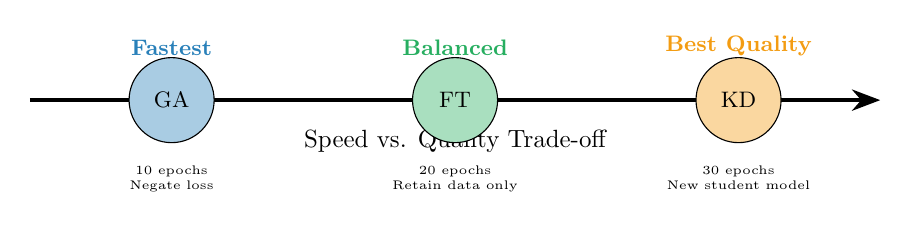
\begin{tikzpicture}[scale=0.9, transform shape]
        % Timeline
        \draw[ultra thick, -Stealth] (-6, 0) -- (6, 0);
        \node[below] at (0, -0.3) {Speed vs. Quality Trade-off};
        
        % VFU-GA
        \node[draw, circle, fill=vflblue!40, minimum size=1.2cm, font=\small] at (-4, 0) {GA};
        \node[above=0.5cm, font=\small\bfseries, vflblue] at (-4, 0) {Fastest};
        \node[below=0.8cm, font=\tiny, text width=2cm, align=center] at (-4, 0) {10 epochs\\Negate loss};
        
        % VFU-FT
        \node[draw, circle, fill=vflgreen!40, minimum size=1.2cm, font=\small] at (0, 0) {FT};
        \node[above=0.5cm, font=\small\bfseries, vflgreen] at (0, 0) {Balanced};
        \node[below=0.8cm, font=\tiny, text width=2cm, align=center] at (0, 0) {20 epochs\\Retain data only};
        
        % VFU-KD
        \node[draw, circle, fill=vflorange!40, minimum size=1.2cm, font=\small] at (4, 0) {KD};
        \node[above=0.5cm, font=\small\bfseries, vflorange] at (4, 0) {Best Quality};
        \node[below=0.8cm, font=\tiny, text width=2.5cm, align=center] at (4, 0) {30 epochs\\New student model};
    \end{tikzpicture}
    \end{center}
    
    \vspace{1em}
    \begin{alertblock}{\faLightbulb\ Our Recommendation}
        \begin{itemize}
            \item Use \textbf{VFU-GA} for quick unlearning when utility loss is acceptable
            \item Use \textbf{VFU-KD} when strong privacy guarantees are required
            \item \textbf{Always verify} with our multi-attack framework!
        \end{itemize}
    \end{alertblock}
\end{frame}

% ============================================================
% SECTION 5: VERIFICATION FRAMEWORK
% ============================================================
\section{Verification: Did We Really Unlearn?}

\begin{frame}{The Critical Question}
    \begin{center}
        {\Large \textbf{How do we VERIFY that unlearning worked?}}
    \end{center}
    
    \vspace{1em}
    \begin{center}
    \begin{tikzpicture}[scale=0.9, transform shape]
        \node[draw, rounded corners, fill=vflblue!30, minimum width=3cm, minimum height=1.2cm, align=center] (mia1) at (-5, 0) {\faSearch\\Output MIA};
        
        \node[draw, rounded corners, fill=vflgreen!30, minimum width=3cm, minimum height=1.2cm, align=center] (mia2) at (-1.7, 0) {\faWaveSquare\\Gradient MIA};
        
        \node[draw, rounded corners, fill=vflorange!30, minimum width=3cm, minimum height=1.2cm, align=center] (fuma) at (1.7, 0) {\faFingerprint\\FUMA};
        
        \node[draw, rounded corners, fill=vflpurple!30, minimum width=3cm, minimum height=1.2cm, align=center] (shadow) at (5, 0) {\faClone\\Shadow Model};
    \end{tikzpicture}
    \end{center}
    
    \vspace{1em}
    \begin{block}{\faShieldAlt\ Why Multiple Attacks?}
        A single attack might miss subtle information leakage.\\
        Our framework uses \textbf{four complementary attacks} for robust verification.
    \end{block}
\end{frame}

\begin{frame}{Attack 1: Output-Based MIA}
    \begin{columns}[T]
        \begin{column}{0.55\textwidth}
            \begin{block}{\faLightbulb\ Intuition}
                Models are more ``confident'' on data they've seen during training!
            \end{block}
            
            \vspace{0.5em}
            \textbf{Features extracted:}
            \begin{enumerate}
                \item Prediction probability $p$
                \item Confidence: $\max(p, 1-p)$
                \item Loss value
                \item Entropy
            \end{enumerate}
        \end{column}
        
        \begin{column}{0.42\textwidth}
            \begin{center}
            \begin{tikzpicture}[scale=0.75, transform shape]
                \node[draw, circle, fill=vflblue!20, minimum size=1.5cm] (model) at (0, 2) {\faBrain};
                \node[draw, rectangle, fill=vflgreen!20, minimum width=1.2cm, font=\small] (input) at (-2.2, 2) {Sample};
                \draw[-{Stealth}, thick] (input) -- (model);
                \node[draw, rectangle, fill=vflorange!20, minimum width=1.5cm, align=center, font=\small] (output) at (0, 0) {$p = 0.95$};
                \draw[-{Stealth}, thick] (model) -- (output);
                \node[draw, rectangle, fill=vflred!20, minimum width=2cm, font=\small] (attack) at (0, -2) {MIA Classifier};
                \draw[-{Stealth}, thick] (output) -- (attack);
            \end{tikzpicture}
            \end{center}
        \end{column}
    \end{columns}
\end{frame}

\begin{frame}{Attack 2: Gradient-Based MIA (Our Contribution)}
    \begin{block}{\faLightbulb\ Key Insight}
        \textbf{Gradients} reveal more than outputs!\\
        They show how the model would \textit{change} given a sample.
    \end{block}
    
    \vspace{0.5em}
    \begin{columns}[T]
        \begin{column}{0.48\textwidth}
            \textbf{Gradient Features (20 total):}
            \begin{itemize}
                \item L2 norm: $||\nabla_\theta||_2$
                \item Layer-wise norms
                \item Statistical moments
                \item Spectral signatures (SVD)
                \item Sparsity ratio
            \end{itemize}
        \end{column}
        
        \begin{column}{0.48\textwidth}
            \begin{exampleblock}{\faChartLine\ Why More Powerful?}
                Gradients capture the model's \textbf{internal reaction} to data, not just surface predictions.
            \end{exampleblock}
        \end{column}
    \end{columns}
\end{frame}

\begin{frame}{Attack 3: FUMA (Forensic Unlearning Attack)}
    \begin{block}{\faFingerprint\ Novel Contribution}
        FUMA detects ``forensic traces'' left by unlearning --- behavioral artifacts that differ between unlearned and never-learned samples.
    \end{block}
    
    \vspace{0.5em}
    \textbf{Method:}
    \begin{enumerate}
        \item Generate \textbf{canary samples} (synthetic probes)
        \item Compute $\Delta_{pred}$ = prediction change before/after unlearning
        \item Train detector on behavioral differences
        \item Test: Can we detect which samples were unlearned?
    \end{enumerate}
    
    \vspace{0.5em}
    \begin{exampleblock}{\faCheck\ Success Criteria}
        Detection rate $<$ 5\% = Effective unlearning\\
        Detection rate $>$ 50\% = Unlearning failed
    \end{exampleblock}
\end{frame}

\begin{frame}{Attack 4: Shadow Model Attack}
    \begin{block}{\faClone\ Concept}
        Train shadow models on retain-only vs full data.\\
        Meta-classifier predicts which distribution trained the model.
    \end{block}
    
    \vspace{0.5em}
    \begin{center}
    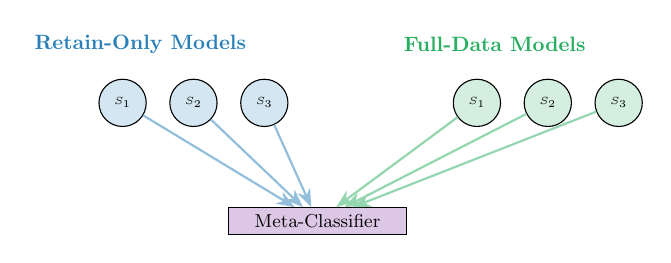
\begin{tikzpicture}[scale=0.75, transform shape]
        \node[font=\bfseries, vflblue] at (-3, 2) {Retain-Only Models};
        \foreach \i in {1,2,3} {
            \node[draw, circle, fill=vflblue!20, minimum size=0.8cm, font=\tiny] (r\i) at ({-4.5+\i*1.2}, 1) {$S_\i$};
        }
        
        \node[font=\bfseries, vflgreen] at (3, 2) {Full-Data Models};
        \foreach \i in {1,2,3} {
            \node[draw, circle, fill=vflgreen!20, minimum size=0.8cm, font=\tiny] (f\i) at ({1.5+\i*1.2}, 1) {$S_\i$};
        }
        
        \node[draw, rectangle, fill=vflpurple!30, minimum width=3cm, font=\small] (meta) at (0, -1) {Meta-Classifier};
        
        \foreach \i in {1,2,3} {
            \draw[-{Stealth}, thick, vflblue!50] (r\i) -- (meta);
            \draw[-{Stealth}, thick, vflgreen!50] (f\i) -- (meta);
        }
    \end{tikzpicture}
    \end{center}
    
    \vspace{0.3em}
    \begin{alertblock}{\faChartLine\ Metric}
        AUC $\approx$ 0.5: Cannot distinguish $\Rightarrow$ Unlearning verified!
    \end{alertblock}
\end{frame}

% ============================================================
% SECTION 6: IMPLEMENTATION
% ============================================================
\section{Our Implementation}

\begin{frame}{Implementation Overview}
    \begin{block}{\faCode\ What We Built in Python/PyTorch}
        \begin{enumerate}
            \item \textbf{VFLDataPartitioner}: Vertically splits features among parties
            \item \textbf{VFLModel}: Split learning with Bottom + Top models
            \item \textbf{VFLTrainer}: Training loop with BCE loss + Adam
            \item \textbf{VFLUnlearner}: GA, FT, KD unlearning methods
            \item \textbf{Verification Framework}: 4 attack implementations
        \end{enumerate}
    \end{block}
    
    \vspace{0.5em}
    \begin{exampleblock}{\faFlask\ Experiment Pipeline}
        Train VFL $\rightarrow$ Select 5\% samples to unlearn $\rightarrow$ Apply unlearning $\rightarrow$ Run verification attacks $\rightarrow$ Measure effectiveness
    \end{exampleblock}
\end{frame}

\begin{frame}{Training Configuration}
    \begin{columns}[T]
        \begin{column}{0.48\textwidth}
            \begin{block}{\faCog\ Model Hyperparameters}
                \begin{itemize}
                    \item Hidden dimension: 64
                    \item Embedding dimension: 32
                    \item Dropout rate: 0.3
                    \item Batch size: 256
                \end{itemize}
            \end{block}
        \end{column}
        
        \begin{column}{0.48\textwidth}
            \begin{block}{\faChartLine\ Training Settings}
                \begin{itemize}
                    \item Epochs: 30-50
                    \item Learning rate: 0.001
                    \item Optimizer: Adam
                    \item Loss: Binary Cross-Entropy
                \end{itemize}
            \end{block}
        \end{column}
    \end{columns}
    
    \vspace{0.5em}
    \begin{block}{\faFlask\ Unlearning Settings}
        \begin{itemize}
            \item Unlearn ratio: 5\% of training samples (1,206 samples for Adult dataset)
            \item VFU-GA: 10 epochs, lr=0.001
            \item VFU-FT: 20 epochs, lr=0.0005
            \item VFU-KD: 30 epochs, T=2.0, $\alpha$=0.5
        \end{itemize}
    \end{block}
\end{frame}

% ============================================================
% SECTION 7: DATASETS
% ============================================================
\section{Datasets}

\begin{frame}{Datasets Overview}
    \begin{table}[]
        \centering
        \large
        \begin{tabular}{lccc}
            \toprule
            \textbf{Dataset} & \textbf{Samples} & \textbf{Features} & \textbf{Parties} \\
            \midrule
            UCI Adult & 30,162 & 14 & 2 \\
            German Credit & 1,000 & 20 & 2 \\
            MIMIC-III & 46,000 & 20 & 3 \\
            \bottomrule
        \end{tabular}
    \end{table}
\end{frame}

\begin{frame}{Dataset Details}
    \begin{columns}[T]
        \begin{column}{0.32\textwidth}
            \begin{block}{\faPeopleArrows\ UCI Adult}
                \begin{itemize}
                    \item Census data
                    \item Task: Income $>$\$50K
                    \item Party A: Demographics
                    \item Party B: Work info
                \end{itemize}
            \end{block}
        \end{column}
        
        \begin{column}{0.32\textwidth}
            \begin{block}{\faCreditCard\ German Credit}
                \begin{itemize}
                    \item Bank data
                    \item Task: Credit risk
                    \item Party A: Account info
                    \item Party B: Personal info
                \end{itemize}
            \end{block}
        \end{column}
        
        \begin{column}{0.32\textwidth}
            \begin{block}{\faHospital\ MIMIC-III}
                \begin{itemize}
                    \item ICU records
                    \item Task: Mortality
                    \item 3 parties: Hospital, Lab, Demographics
                \end{itemize}
            \end{block}
        \end{column}
    \end{columns}
\end{frame}

% ============================================================
% SECTION 7: RESULTS
% ============================================================
\section{Experimental Results}

\begin{frame}{Model Performance Results}
    \begin{columns}[T]
        \begin{column}{0.48\textwidth}
            \begin{block}{\faChartBar\ UCI Adult Results}
                \begin{table}[]
                    \centering
                    \begin{tabular}{lcc}
                        \toprule
                        \textbf{Metric} & \textbf{Before} & \textbf{After} \\
                        \midrule
                        Accuracy & 85.1\% & 80.9\% \\
                        F1 Score & 0.684 & 0.668 \\
                        AUC & 0.910 & 0.893 \\
                        \bottomrule
                    \end{tabular}
                \end{table}
            \end{block}
            
            \textcolor{vflgreen}{\faCheckCircle} \textbf{Utility drop: 4.9\%} (acceptable)
        \end{column}
        
        \begin{column}{0.48\textwidth}
            \begin{block}{\faShieldAlt\ Verification Results}
                \begin{table}[]
                    \centering
                    \begin{tabular}{lc}
                        \toprule
                        \textbf{Attack} & \textbf{Metric} \\
                        \midrule
                        Output MIA AUC & 0.516 \\
                        Gradient MIA AUC & 0.537 \\
                        Unlearn Effectiveness & 50.1\% \\
                        FUMA Detection & 63.5\% \\
                        \bottomrule
                    \end{tabular}
                \end{table}
            \end{block}
        \end{column}
    \end{columns}
\end{frame}

\begin{frame}{MIA Results: Output-Based Attack}
    \begin{columns}[T]
        \begin{column}{0.55\textwidth}
            \begin{center}
                \includegraphics[width=\textwidth]{mia_results.png}
            \end{center}
        \end{column}
        \begin{column}{0.42\textwidth}
            \begin{block}{\faChartBar\ Reading the Graph}
                \small
                \begin{itemize}
                    \item \textbf{Y-axis}: Classification rate (\%)
                    \item \textbf{3 bars}: Members, Non-Members, Unlearned
                    \item \textbf{Dashed line}: Random guess (50\%)
                \end{itemize}
            \end{block}
        \end{column}
    \end{columns}
\end{frame}

\begin{frame}{MIA Results: Interpretation}
    \begin{block}{\faSearch\ What The Bars Show}
        \begin{itemize}
            \item \textbf{Members (Red, 64.9\%)}: Attack correctly identifies training samples
            \item \textbf{Non-Members (Blue, 37.3\%)}: Attack incorrectly classifies test samples
            \item \textbf{Unlearned (Green, 50.1\%)}: Attack is \textbf{confused} --- close to random!
        \end{itemize}
    \end{block}
    
    \vspace{0.5em}
    \begin{exampleblock}{\faCheck\ Key Insight}
        \textbf{Goal}: Unlearned samples should look like non-members.
        \begin{itemize}
            \item Unlearned rate (50.1\%) is \textbf{between} members and non-members
            \item Attack can't confidently classify unlearned samples
            \item \textbf{Partial success}: Model has ``partially forgotten'' the data
        \end{itemize}
    \end{exampleblock}
\end{frame}

\begin{frame}{Gradient MIA: Comparison Results}
    \begin{columns}[T]
        \begin{column}{0.55\textwidth}
            \begin{center}
                \includegraphics[width=\textwidth]{gradient_mia_comparison.png}
            \end{center}
        \end{column}
        \begin{column}{0.42\textwidth}
            \begin{block}{\faWaveSquare\ Reading the 3 Plots}
                \small
                \begin{itemize}
                    \item \textbf{Left}: Attack AUC\\(higher = more info leaked)
                    \item \textbf{Middle}: Unlearning effectiveness (\%)
                    \item \textbf{Right}: Gradient change distribution
                \end{itemize}
            \end{block}
        \end{column}
    \end{columns}
\end{frame}

\begin{frame}{Gradient MIA: Interpretation}
    \begin{block}{\faChartBar\ Comparing the Two Attack Methods}
        \begin{itemize}
            \item \textbf{Output MIA AUC: 0.516} --- slightly above random (0.5)
            \item \textbf{Gradient MIA AUC: 0.464} --- slightly below random
            \item \textbf{Effectiveness}: Both $\approx$50\% (50.1\% vs 50.2\%)
        \end{itemize}
    \end{block}
    
    \vspace{0.3em}
    \begin{exampleblock}{\faLightbulb\ Key Insights}
        \begin{itemize}
            \item Both attacks near \textbf{random performance} $\Rightarrow$ unlearning works!
            \item \textbf{Gradient changes} (Mean: 39.56) show model parameters shifted
            \item This proves the model \textbf{internally changed} after unlearning
        \end{itemize}
    \end{exampleblock}
    
    \vspace{0.3em}
    \begin{alertblock}{\faExclamationTriangle\ Why Both Methods Matter}
        Output MIA alone may miss subtle information leakage. Gradient-based analysis provides \textbf{deeper verification} of internal model changes.
    \end{alertblock}
\end{frame}

\begin{frame}{Gradient Feature Importance}
    \begin{columns}[T]
        \begin{column}{0.55\textwidth}
            \begin{center}
                \includegraphics[width=\textwidth]{gradient_feature_importance.png}
            \end{center}
        \end{column}
        \begin{column}{0.42\textwidth}
            \begin{block}{\faSearchPlus\ Reading the Graph}
                \small
                \begin{itemize}
                    \item \textbf{Horizontal bars}: Feature importance scores
                    \item \textbf{Random Forest} classifier ranks features
                    \item Longer bar = more discriminative
                \end{itemize}
            \end{block}
        \end{column}
    \end{columns}
\end{frame}

\begin{frame}{Feature Importance: Interpretation}
    \begin{block}{\faChartBar\ Top Features for Membership Inference}
        \small
        \begin{columns}[T]
            \begin{column}{0.48\textwidth}
                \begin{enumerate}
                    \item \textbf{Grad Direction Std} (0.08)
                    \item \textbf{Grad Direction Mean} (0.075)
                    \item \textbf{Sparsity} (0.074)
                    \item \textbf{Grad Mean} (0.07)
                    \item \textbf{Bottom Model 1 Norm} (0.065)
                \end{enumerate}
            \end{column}
            \begin{column}{0.48\textwidth}
                \begin{enumerate}
                    \setcounter{enumi}{5}
                    \item \textbf{Bottom Model 2 Norm} (0.063)
                    \item \textbf{Grad Max} (0.062)
                    \item \textbf{Spectral Val 2} (0.061)
                    \item \textbf{Percentile 75} (0.059)
                    \item \textbf{Grad Min} (0.056)
                \end{enumerate}
            \end{column}
        \end{columns}
    \end{block}
    
    \vspace{0.3em}
    \begin{exampleblock}{\faLightbulb\ What This Tells Us}
        \begin{itemize}
            \item \textbf{Gradient direction} (std, mean) most informative --- captures \textit{how} model would update
            \item \textbf{Bottom model norms}: Per-party gradient magnitudes reveal local model reactions
            \item \textbf{Sparsity}: Training samples cause more sparse gradient patterns
        \end{itemize}
    \end{exampleblock}
\end{frame}

\begin{frame}{FUMA: Forensic Results}
    \begin{columns}[T]
        \begin{column}{0.55\textwidth}
            \begin{center}
                \includegraphics[width=\textwidth]{fuma_results.png}
            \end{center}
        \end{column}
        \begin{column}{0.42\textwidth}
            \begin{block}{\faFingerprint\ Reading the 4 Plots}
                \small
                \begin{itemize}
                    \item \textbf{Top-Left}: Canary attack results (3 types)
                    \item \textbf{Top-Right}: Forensic feature importance
                    \item \textbf{Bottom-Left}: Detection rate gauge
                    \item \textbf{Bottom-Right}: Feature comparison
                \end{itemize}
            \end{block}
        \end{column}
    \end{columns}
\end{frame}

\begin{frame}{FUMA: Interpretation (Part 1)}
    \begin{block}{\faChartBar\ Canary Attack Results (Top-Left)}
        Three types of canary samples tested:
        \begin{itemize}
            \item \textbf{Extreme}: Highest divergence ($\approx$0.11) --- most detectable
            \item \textbf{Boundary}: Lower divergence ($\approx$0.05) --- harder to detect
            \item \textbf{Interpolated}: Similar to boundary ($\approx$0.05)
        \end{itemize}
        Red dashed line (0.10) = detection threshold
    \end{block}
    
    \vspace{0.3em}
    \begin{alertblock}{\faExclamationTriangle\ Detection Rate: 63.5\% (Bottom-Left Gauge)}
        \begin{itemize}
            \item \textbf{Green zone} ($<$5\%): Excellent unlearning
            \item \textbf{Yellow zone} (5-50\%): Moderate
            \item \textbf{Red zone} ($>$50\%): Poor --- \textbf{we are here!}
        \end{itemize}
    \end{alertblock}
\end{frame}

\begin{frame}{FUMA: Interpretation (Part 2)}
    \begin{block}{\faSearchPlus\ Top Forensic Features (Top-Right)}
        Features that best distinguish unlearned samples:
        \begin{itemize}
            \item \textbf{grad\_sign\_flip\_ratio} (0.175): Gradient direction changes
            \item \textbf{grad\_direction\_change} (0.19): How gradients rotate
            \item \textbf{pred\_stability} (0.16): Prediction consistency
            \item \textbf{grad\_magnitude\_ratio} (0.12): Gradient size changes
        \end{itemize}
    \end{block}
    
    \vspace{0.3em}
    \begin{exampleblock}{\faChartBar\ Feature Comparison (Bottom-Right)}
        Compares \textcolor{red}{Unlearned} vs \textcolor{blue}{Retained} samples:
        \begin{itemize}
            \item \textbf{grad\_magnitu}: Largest difference --- unlearned samples show \textbf{much higher} gradient magnitude changes
            \item \textbf{grad\_abs\_cha}: Second largest difference
            \item These are \textbf{forensic traces} left by the unlearning process
        \end{itemize}
    \end{exampleblock}
\end{frame}

\begin{frame}{FUMA: Conclusion}
    \begin{alertblock}{\faExclamationTriangle\ Critical Finding}
        VFU-GA leaves \textbf{detectable forensic traces}:
        \begin{itemize}
            \item 63.5\% detection rate is \textbf{much higher} than the 5\% target
            \item Unlearned samples have systematically different gradient behaviors
            \item An adversary can distinguish ``unlearned'' from ``never-learned'' samples
        \end{itemize}
    \end{alertblock}
    
    \vspace{0.5em}
    \begin{exampleblock}{\faLightbulb\ Practical Recommendation}
        \begin{itemize}
            \item For applications requiring \textbf{strong privacy guarantees}, use \textbf{VFU-KD} instead of VFU-GA
            \item VFU-KD produces more natural-looking model behavior
            \item Trade-off: VFU-KD is slower but leaves fewer artifacts
        \end{itemize}
    \end{exampleblock}
\end{frame}

\begin{frame}{Key Findings: Summary}
    \begin{block}{\faChartBar\ Quantitative Results}
        \begin{table}
            \small
            \begin{tabular}{l c c}
                \textbf{Metric} & \textbf{Value} & \textbf{Interpretation} \\
                \hline
                Output MIA AUC & 0.516 & Near random (good) \\
                Gradient MIA AUC & 0.464 & Near random (good) \\
                Unlearn Classification & 50.1\% & Partial forgetting \\
                FUMA Detection & 63.5\% & \textcolor{red}{High (bad)} \\
            \end{tabular}
        \end{table}
    \end{block}
    
    \vspace{0.3em}
    \begin{columns}[T]
        \begin{column}{0.48\textwidth}
            \begin{exampleblock}{\faCheck\ Good News}
                \begin{itemize}
                    \item MIA attacks near random
                    \item Model outputs don't leak
                    \item Basic unlearning works
                \end{itemize}
            \end{exampleblock}
        \end{column}
        \begin{column}{0.48\textwidth}
            \begin{alertblock}{\faExclamationTriangle\ Concern}
                \begin{itemize}
                    \item FUMA detects artifacts
                    \item Gradient forensics reveal traces
                    \item Stronger methods needed
                \end{itemize}
            \end{alertblock}
        \end{column}
    \end{columns}
\end{frame}

% ============================================================
% SECTION 8: CONCLUSION
% ============================================================
\section{Conclusion}

\begin{frame}{Complete Workflow}
    \begin{center}
    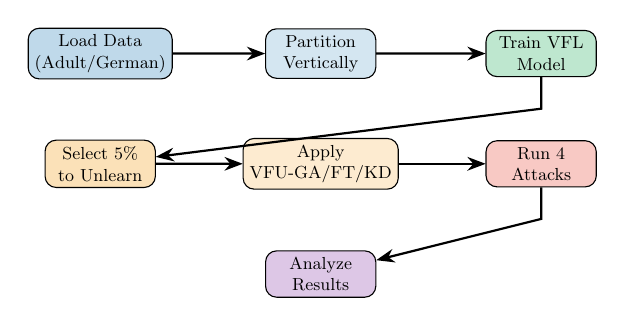
\begin{tikzpicture}[scale=0.7, transform shape,
        box/.style={draw, rounded corners, minimum width=2cm, minimum height=0.8cm, font=\small, align=center}]
        
        % Row 1: Data
        \node[box, fill=vflblue!30] (data) at (0, 4) {Load Data\\(Adult/German)};
        \node[box, fill=vflblue!20] (partition) at (4, 4) {Partition\\Vertically};
        \node[box, fill=vflgreen!30] (train) at (8, 4) {Train VFL\\Model};
        
        % Row 2: Unlearning
        \node[box, fill=vflorange!30] (select) at (0, 2) {Select 5\%\\to Unlearn};
        \node[box, fill=vflorange!20] (unlearn) at (4, 2) {Apply\\VFU-GA/FT/KD};
        \node[box, fill=vflred!30] (verify) at (8, 2) {Run 4\\Attacks};
        
        % Row 3: Results
        \node[box, fill=vflpurple!30] (results) at (4, 0) {Analyze\\Results};
        
        % Arrows
        \draw[-{Stealth}, thick] (data) -- (partition);
        \draw[-{Stealth}, thick] (partition) -- (train);
        \draw[-{Stealth}, thick] (train) -- (8, 3) -- (select);
        \draw[-{Stealth}, thick] (select) -- (unlearn);
        \draw[-{Stealth}, thick] (unlearn) -- (verify);
        \draw[-{Stealth}, thick] (verify) -- (8, 1) -- (results);
    \end{tikzpicture}
    \end{center}
    
    \vspace{0.3em}
    \begin{block}{\faClipboardCheck\ Output}
        Model performance (accuracy, F1, AUC) + Verification metrics (MIA AUC, FUMA detection, effectiveness scores)
    \end{block}
\end{frame}

\begin{frame}{What We Built}
    \begin{block}{\faCode\ E-VFU Framework Components}
        \begin{enumerate}
            \item \textbf{VFL Architecture}: Split learning with Bottom + Top models
            \item \textbf{Three Unlearning Methods}:
            \begin{itemize}
                \item VFU-GA: Gradient Ascent (fast, strong forgetting)
                \item VFU-FT: Fine-Tuning (balanced approach)
                \item VFU-KD: Knowledge Distillation (best quality)
            \end{itemize}
            \item \textbf{Multi-Attack Verification}:
            \begin{itemize}
                \item Output MIA + \textbf{Gradient MIA} (novel)
                \item \textbf{FUMA} (novel for VFL) + Shadow Model Attack
            \end{itemize}
        \end{enumerate}
    \end{block}
\end{frame}

\begin{frame}{Key Takeaways}
    \begin{exampleblock}{\faLightbulb\ Key Findings}
        \begin{itemize}
            \item Gradient-MIA reveals more than output-MIA
            \item FUMA detects forensic traces of unlearning
            \item VFU-KD provides strongest forgetting guarantees
            \item Multi-attack verification is essential
        \end{itemize}
    \end{exampleblock}
    
    \vspace{1em}
    \begin{alertblock}{\faRoad\ Future Work}
        \begin{itemize}
            \item Certified unlearning bounds
            \item Defense against verification attacks
            \item Larger-scale experiments
        \end{itemize}
    \end{alertblock}
\end{frame}

\begin{frame}{Validation Dashboard}
    \begin{center}
    \begin{tikzpicture}[scale=0.9, transform shape]
        \node[font=\Large\bfseries] at (0, 3.5) {Verification Thresholds};
        
        \begin{scope}[shift={(-4, 1)}]
            \node[font=\small\bfseries] at (0, 1.5) {MIA AUC};
            \fill[vflgreen!60] (0,0) circle (1);
            \node[font=\large, white] at (0, 0) {0.52};
            \node[font=\small, vflgreen] at (0, -1.5) {\faCheck\ PASS};
        \end{scope}
        
        \begin{scope}[shift={(0, 1)}]
            \node[font=\small\bfseries] at (0, 1.5) {Effectiveness};
            \fill[vflgreen!60] (0,0) circle (1);
            \node[font=\large, white] at (0, 0) {50\%};
            \node[font=\small, vflgreen] at (0, -1.5) {\faCheck\ PASS};
        \end{scope}
        
        \begin{scope}[shift={(4, 1)}]
            \node[font=\small\bfseries] at (0, 1.5) {FUMA Rate};
            \fill[vflred!60] (0,0) circle (1);
            \node[font=\large, white] at (0, 0) {63\%};
            \node[font=\small, vflred] at (0, -1.5) {\faTimes\ FAIL};
        \end{scope}
    \end{tikzpicture}
    \end{center}
    
    \vspace{0.5em}
    \centering
    \colorbox{yellow!20}{\textbf{Verdict:} VFU-GA achieves basic unlearning, but FUMA reveals detectable artifacts.}
\end{frame}

\begin{frame}[standout]
    \centering
    {\Huge Thank You!}
    
    \vspace{1em}
    {\large Questions?}
    
    \vspace{2em}
    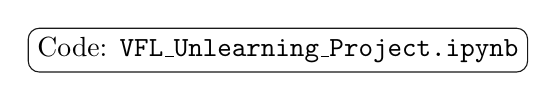
\begin{tikzpicture}
        \node[draw, rounded corners, fill=white, opacity=0.9, text opacity=1] {
            Code: \texttt{VFL\_Unlearning\_Project.ipynb}
        };
    \end{tikzpicture}
\end{frame}

% ============================================================
% BACKUP SLIDES
% ============================================================
\appendix

\begin{frame}{Appendix: HFL vs VFL Comparison}
    \begin{table}[]
        \centering
        \footnotesize
        \begin{tabular}{p{2.5cm}p{4.5cm}p{4.5cm}}
            \toprule
            \textbf{Aspect} & \textbf{HFL Unlearning} & \textbf{VFL Unlearning} \\
            \midrule
            Data Distribution & Samples across clients & Features across parties \\
            Unlearning Target & Client data / samples & Client features / samples \\
            Communication & Gradients to server & Embeddings between parties \\
            Key Methods & FedEraser, SISA, FRU & VFU-GA, VFU-KD, VFU-LR \\
            \bottomrule
        \end{tabular}
    \end{table}
\end{frame}

\begin{frame}{Appendix: References}
    \footnotesize
    \textbf{VFL Unlearning:}
    \begin{itemize}
        \item Varshney et al. (2025): VFU-KD/VFU-GA
        \item Deng et al. (2023): VFU-LR
        \item Wang \& Wang (2025): Certified VFL unlearning
    \end{itemize}
    
    \vspace{0.3em}
    \textbf{HFL Unlearning:}
    \begin{itemize}
        \item Liu et al. (2021): FedEraser
        \item Bourtoule et al. (2021): SISA
    \end{itemize}
    
    \vspace{0.3em}
    \textbf{Membership Inference:}
    \begin{itemize}
        \item Shokri et al. (2017): Shadow model MIA
        \item Geiping et al. (2020): Gradient-based attacks
    \end{itemize}
\end{frame}

\end{document}
